\documentclass{article}

\def\subj {MATH}
\def\npart {412}
\def\nterm {Fall}
\def\nyear {2018}
\def\ncourse {Partial Differential Equations}



\input{header}

\setlength\parindent{0pt}

\begin{document}
\maketitle
{\small
  \noindent\textbf{Heat Equation}\\
  Conduction of Heat in a 1-Dimensional rod, boundary conditions, equilibrium temperature distribution, heat condition in 2 or 3 dimensions.\hspace*{\fill} [1]

  \vspace{10pt}
  \noindent\textbf{Method of Separation of Variables}\\
  Linearity, heat equation with zero temperatures at finite ends, orthogonality of functions, Laplace's equation; solutions and qualitative properties.\hspace*{\fill} [2]

  \vspace{10pt}
  \noindent\textbf{Fourier Series}\\
  Statement of Convergence Theorem, Fourier cosine and sine series, term-by-term differentiation of Fourier series, term-by-term integration of Fourier series, complex form of Fourier series.\hspace*{\fill} [3]

  \vspace{10pt}
  \noindent\textbf{Wave Equation}\\
  Vertically vibrating string, boundary conditions, vibrating string with fixed ends, vibrating membrane, reflection and refraction of electromagnetic and acoustic sound waves.\hspace*{\fill} [4]
  
  \vspace{10pt}
  \noindent\textbf{The Method of Characteristics for Linear and Quasilinear
  	Wave Equations}\\
  Characteristics for first order wave equations, method of characteristics for first order PDEs, one-dimensional wave equation, a vibrating string of fixed length, many quasilinear PDEs, semi-infinite strings and reflections. \hspace*{\fill} [12]
  
  \vspace{10pt}
  \noindent\textbf{Fourier Transform Solutions of Partial
  	Differential Equations}\\
  Heat equation on an infinite domain, Fourier transform pair, inverse Fourier transform, convolution theorem.\hspace*{\fill} [10]

  \vspace{10pt}
  \noindent\textbf{Green’s Functions for Time-Independent Problems}\\
  Green's functions for boundary value problems for ODEs, method of eigenvalue expansion, nonhomogeneous boundary conditions.\hspace*{\fill} [9]}

\tableofcontents


	\section{The Heat Equation}
	
	\subsection{Introduction}
	
	In this course we will learn to find solutions of elementary problems involving partial differential equations, the kinds of problems that arise in various fields of science and engineering. A \textit{partial differential equation} (PDE) is a mathematical equation involving a function and its partial derivatives, for example,
	\[
		\frac{\partial u}{\partial t} + 3\frac{\partial u}{\partial x} = 0
	\]
	is a PDE of the function $ u(x,t) $.
	
	\subsection{Derivation of the Heat Equation in a 1-D Rod}
	
	Heat flows in a body in two main ways:
	\begin{enumerate}[label=(\arabic*)]
		\item Conduction: Kinetic energy is transferred from one molecule to another.
		\item Convection: Movement of molecules themselves transfer heat.
	\end{enumerate}
	
	We will only be looking at conduction.

	\begin{center}
		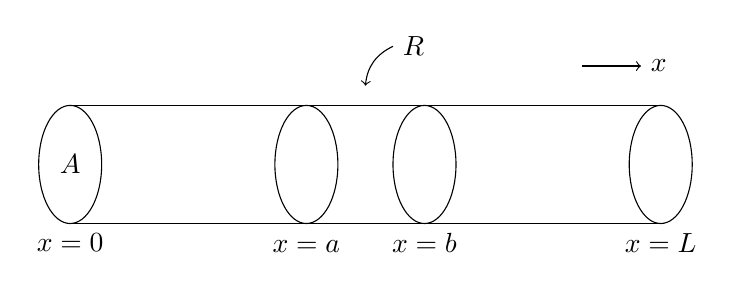
\begin{tikzpicture}
			\draw (0,0) ellipse (0.4cm and 0.75cm);
			\draw (0,0.75) -- (3,0.75);
			\draw (0,-0.754) -- (3,-0.754);
			\draw (3,0) ellipse (0.4cm and 0.75cm);
			
			\draw (4.5,0) ellipse (0.4cm and 0.75cm);
			\draw (3,0.75) -- (4.5,0.75);
			\draw (3,-0.754) -- (4.5,-0.754);
			
			\draw (7.5,0) ellipse (0.4cm and 0.75cm);
			\draw (4.5,0.75) -- (7.5,0.75);
			\draw (4.5,-0.754) -- (7.5,-0.754);
			
			\node at (0,0) {$ A $};
			\node at (0,-0.75) [below] {$ x=0 $};
			\node at (3,-0.84) [below] {$ x=a $};
			\node at (4.5,-0.75) [below] {$ x=b $};
			\node at (7.5,-0.75) [below] {$ x=L $};
			
			\draw [->] (6.5,1.25) -- (7.25,1.25) node[right] {$x$};
			\draw [<-] (3.75,1) to[bend left] (4.1,1.5) node[right] {$R$};
		\end{tikzpicture}
	\end{center}
	
	The cross sectional area $ A $ is constant. Let $ e(x,t) $ which is the thermal energy density have units energy/value. Assume that all thermal quantities are constant across cross-sections. Also, all quantities depend on $ x,t $ only; and the sides of the rod are perfectly insulated. \\
	
	Then the heat energy in $ R $ at time $ t $ is given by:
	\[
		\int_a^b Ae(x,t) \, dx
	\]
	
	\textbf{Conservation of Energy} \\
	
	Heat energy on $ R $ changes by:
	\begin{enumerate}[label=(\arabic*)]
		\item Flow in/out of ends at $ x=a,b $.
		\item Generated inside of $ R $.
	\end{enumerate}
	
	The heat flux, given by $ \phi(x,t) $, is the thermal energy/unit time/unit surface area. Heat flowing to the right is given by $ \phi(x,t) > 0 $, and $ \phi(x,t) < 0 $ indicates that heat flows to the left. \\
	
	The heat flux in and out of $ R $ is given by
	\[
		\phi(a,t)A - \phi(b,t)A = A(\phi(a,t) - \phi(b,t))
	\]
	A heat source $ Q(x,t) $ is the heat energy generated/unit volume/unit time.
	
	The exact conservation of energy is given by
	\[
		\frac{d}{dt} \int_a^b Ae(x,t) \, dx = A(\phi(a,t) - \phi(b,t)) + \int_a^b AQ(x,t) \, dx
	\]
	
	Note that by using the Fundamental Theorem of Calculus,
	\[
		\phi(a,t) - \phi(b,t) = -\int_a^b \frac{\partial \phi}{\partial x} \, dx
	\]
	and
	\[
		\frac{d}{dt} \int_a^b e(x,t) \, dx = \int_a^b \frac{\partial e}{\partial t} \, dx
	\]
	Thus,
	\[
		\int_a^b \left( \frac{\partial e}{\partial t} + \frac{\partial \phi}{\partial x} - Q \right)A \, dx = 0 \quad \text{for all } a,b.
	\]
	Which means that the integrand must be 0:
	\begin{align*}
		&\frac{\partial e}{\partial t} + \frac{\partial \phi}{\partial x} - Q = 0 \quad \text{or,} \\
		&\frac{\partial e}{\partial t} = - \frac{\partial \phi}{\partial x} + Q
	\end{align*}
	where $ u(x,t) $ is temperature in the rod at a position $ x $ and time $ t $. \\
	
	\textbf{Specific Heat}: Denoted by $ c $ is the heat energy necessary to raise temperature of a unit mass by one temperature unit. It has units energy/(mass $ \times $ temp). Note that $ c $ depends on material \underline{and} temperature. Something like $ c = c(x,u(x,t)) $ which makes the above PDE nonlinear. So to simplify, things, we assume $ c=c(x) $ only. \\
	
	The total thermal energy in $ R $ is then
	\[
		\int_a^b e(x,t)A \, dx = \int_a^b cu(x,t) \rho \, dx
	\]
	where $ \rho = $ mass density (mass/unit volume). \\
	
	Thus $ e(x,t) = cu\rho $, and
	\[
		c(x) \rho(x) \frac{\partial u}{\partial t} = -\frac{\partial \phi}{\partial x} + Q
	\]
	\\
	Qualitative properties of heat flow:
	\begin{enumerate}[label=(\arabic*)]
		\item No energy flow if temperature is constant.
		\item Heat flows from hotter to colder regions.
		\item Greater temperature difference implies there is more heat flow.
		\item Rate of heat flow is material dependent.
	\end{enumerate}

	\textbf{Fourier's Law}: The heat flux $ \phi = -K_0 \frac{\partial u}{\partial x} $, where $ K $ is thermal conductivity (small $ K $ means good insulator). Substituting this in, we get the following PDE. \\
	
	\textbf{The Heat Equation}
	
	\[
		c \rho \frac{\partial u}{\partial t} = \frac{\partial}{\partial x} \left( K_0 \frac{\partial u}{\partial x} \right) + Q
	\]
	$ Q,c,\rho,K_0 $ are all given (material properties). The temperature $ u(x,t) $ is unknown. \\
	
	If $ c,\rho, K $ are constant, then the PDE becomes
	\[
		\frac{\partial u}{\partial t} = k \frac{\partial^2 u}{\partial u^2} + Q.
	\]
	Let $ k = K_0/c\rho $ (thermal diffusivity) such that 
	\[
		\frac{\partial u}{\partial t} = k \frac{\partial^2 u}{\partial x^2} + Q
	\]
	or
	\[
		\frac{\partial u}{\partial t} - k\frac{\partial^2 u}{\partial x^2} = Q
	\]
	
	\subsection{Boundary Conditions}
	
	Along with initial conditions, boundary conditions are needed to obtain a well-posed problem (one that has a unique solution). \\
	
	In the case of the 1-D rod, boundary conditions are posed at $ x=0 $ and $ x=L $. We then have three different options: \\
	
	\textbf{Option 1}: Fix temperature boundary conditions:
	\[
		u(0,t) = u_B(t)
	\]
	where $ u_B(t) $ is given and at the left end of the rod. The function $ u_B(t) $ is imposed by placing a reservoir at the left end, e.g. an ice bath. \\
	
	\textbf{Option 2}: Prescribe heat flow at the boundary:
	\[
		-k(0) \frac{\partial u}{\partial x}(0,t) = \phi(t)
	\]
	Simplest example: Perfectly insulated boundary.
	\[
		\frac{\partial u}{\partial x}(0,t) = 0
	\]
	We can also prescribe similar conditions at $ x=L $. \\
	
	\textbf{Option 3}: Newton's Law of Cooling \\
	
	Heat flow leaving the rod is proportional to the temperature difference between the rod and surrounding medium.
	\[
		-k(0) \frac{\partial u}{\partial x}(0,t) = -H(u(0,t) - u_B(0,t))
	\]
	where $ u_B $ is the temperature of the external medium and $ H $ is the heat transfer coefficient. If $ u(0,t) > u_B(t) $ then $ \frac{\partial u}{\partial x} > 0 $, i.e, temperature increases from left to right. Heat flows \underline{out} of the rod. \\
	
	At $ x=L $,
	\[
		-k(L) \frac{\partial u}{\partial x}(L,t) = H(u(L,t) - u_B(t))
	\]
	
	\textbf{Note}: As $ H \to 0 $, there is little energy distribution, and we end up with a perfectly insulated rod. As $ H \to \infty $, $ u(0,t) = u_B(t) $. \\
	
	\textbf{Note}: We can prescribe different types of boundary conditions at each end.
	
	\subsection{Equilibrium Temperature Distribution}
	
	\subsubsection{Prescribed Temperature}
	
	Assume constant thermal properties, $ Q=0 $, and prescribed temperature. Then we have the following PDE:
	\[
		\begin{cases}
			\dfrac{\partial u}{\partial t} = k \dfrac{\partial^2 u}{\partial x^2} \vspace{1mm} \\
			u(0,t) = T_1(t) \\
			u(L,t) = T_2(t) \\
			u(x,0) = f(x)
		\end{cases}
	\]
	At equilibrium, $ u(x,t) $ does not change, i.e $ \frac{\partial u}{\partial t} = 0 $. \\
	
	Our goal is to find equilibrium solutions (temperature distributions that don't change in time). So assume $ u(0,t) = T_1, u(L,t) = T_2 $ and that $ T_1, T_2 $ are constant. So we end up with
	\[
		\frac{\partial^2 u}{\partial x^2} = 0
	\]
	after integrating twice we find that $ u(x,t) = c_1 x + c_2 $.
	
	\begin{center}
		\begin{tikzpicture}
			\draw (-0.25,0) -- (4,0) node[right] {$x$};
			\draw (0,-0.25) -- (0,2) node[left] {$t$};
			\draw (2.75,-0.1) -- (2.75,0.1) node[below=2mm] {$L$};
			\draw (-0.1,0.5) -- (0.1,0.5) node[left=1.5mm] {$T_1$};
			\draw (-0.1,1.4) -- (0.1,1.4) node[left=1.5mm] {$T_2$};
			\node[circle,draw=black, fill=black, inner sep=0pt,minimum size=2pt] (a) at (0,0.5) {};
			\node[circle,draw=black, fill=black, inner sep=0pt,minimum size=2pt] (b) at (2.75,1.4) {};
			\draw[thick] (a) -- (b) node[right] {$u(x,t)$};
		\end{tikzpicture}
	\end{center}
	Solving for $ c_1, c_2 $, we obtain a solution for $ u(x,t) $.
	\[
		u(x,t) = \frac{T_2 - T_1}{L} x + T_1
	\]
	We expect that
	\[
		\lim\limits_{t \to \infty} u(x,t) = \frac{T_2 - T_1}{L} x + T_1
	\]
	no matter what $ f(x) = u(x,0) $ is.
	
	
	\subsubsection{Perfectly Insulated Ends}
	
	If we still assume constant thermal properties, $ Q = 0 $, and prescribed temperature but with the added condition that 
	\[
		\frac{\partial u}{\partial x}(0,t) = \frac{\partial u}{\partial x}(L,t) = 0
	\]
	then we have the following PDE:
	\[
		\begin{cases}
			\dfrac{\partial u}{\partial t} = k \dfrac{\partial^2 u}{\partial x^2} \vspace{1mm} \\
			u(x,0) = f(x) \vspace{1mm} \\
			\dfrac{\partial u}{\partial x}(0,t) = 0 \vspace{1mm} \\
			\dfrac{\partial u}{\partial x}(L,t) = 0
		\end{cases}
	\]
	Like before,
	\[
		\frac{\partial u}{\partial t} = 0 \Rightarrow \frac{\partial^2 u}{\partial x^2} = 0 \Rightarrow u(x,t) = c_1x + c_2
	\]
	So $ \frac{\partial u}{\partial x} = c_1 $, but our first boundary condition says that $ \frac{\partial u}{\partial x}(0,t) = 0 $, so that means that $ c_1=0 $. Thus $ u(x,t) = c_2 $ which implies that equilibrium temperature distribution is constant. All we need to do now is to find $ c_2 $. \\
	
	To find $ c_2 $, we first note that the total heat energy in the rod is given by
	\begin{align*}
		\frac{d}{dt} \int_0^L c\rho u(x,t) \, dx &= \int_0^L c\rho \frac{\partial u}{\partial x}(x,t) \, dx \\
		&= \int_0^L c \rho k \frac{\partial^2 u}{\partial x^2} \, dx \\
		&= c\rho k \left( \frac{\partial u}{\partial x}(L,t) - \frac{\partial u}{\partial x}(0,t) \right) = 0
	\end{align*}
	Since the total heat energy in the rod does not change,
	\begin{align*}
		\int_0^L c \rho u(x,t) \, dx &= \int_0^L c \rho u(x,0) \, dx \\
		&= c \rho \int_0^L f(x) \, dx
	\end{align*}
	Our equilibrium solution is then $ u(x) = c_2 $,
	\begin{align*}
		&\int_0^L c_2 \, dx = \int_0^L f(x) \, dx \\
		&\Rightarrow c_2 = \frac{1}{L} \int_0^L f(x) \, dx.
	\end{align*}
	
	
	\subsection{The Heat Equation in 2 or 3 Dimensions}
	
	In one dimension we had 
	\[
		\frac{\partial u}{\partial t} = k\frac{\partial^2 u}{\partial x^2}
	\]
	where $ u=u(x,t) $ was our temperature. In 3 dimensions we now have something like $ u = u(t,x,y,z) $.\\
	
	Let $ R $ be a 3-D region. Recall that the rate of change of heat energy in $ R $ is the heat flow across the boundary plus the heat generated inside per unit time. The heat energy in $ R $ is given by
	\[
		\int_R c\rho u(t,x,y,z) \, dV
	\]
	where $ c $ is the specific heat and $ \rho $ is the mass density.
	
	\begin{center}
		\begin{tikzpicture}[use Hobby shortcut,closed=true,scale=0.4]
			\draw (-3.5,0.5) .. (-3,2.5) .. (-1,3.5).. (1.5,3).. (4,3.5).. (5,2.5).. (5,0.5) ..(2.5,-2).. (0,-0.5).. (-3,-2).. (-3.5,0.5);
			\node at (-0.5,2) {$R$};
			\draw[thick,->] (1,3) -- (1.5,5) node[below left=2mm] {$\mathbf{n}$};
			\draw[thick,->] (1,3) -- (4,4.5) node[right] {$\bm{\phi}$};
			\node at (5.5,-1) {$\partial R$};
		\end{tikzpicture}
	\end{center}
	Where $ \partial R $ is the boundary (edge) of the region $ R $, $ \mathbf{n} $ is the unit normal vector, and $ \bm{\phi} $ is the heat flux vector. So the heat flux across $ \partial R $ is then given by $ -\bm{\phi} \cdot \mathbf{n} $, this is flowing \underline{into} $ R $. Thus
	\[
		\frac{d}{dt} \int_R c \rho u(t,x,y,z) \, dV = -\int_{\partial R} \bm{\phi} \cdot \mathbf{n} \, dS + \int_R Q \, dV
	\]
	where $ Q = Q(t,x,y,z) $ is the heat source.
	
	\textbf{Divergence Theorem/Vector Calc Review} \\
	
	Recall the gradient operator on a function $ u(x,y,z) $
	\[
		\nabla u(x,y,z) = \frac{\partial u}{\partial x} \ihat + \frac{\partial u}{\partial y} \jhat + \frac{\partial u}{\partial z} \khat 
	\]
	where $ \ihat, \jhat, \khat $ are the standard unit basis vectors in the Cartesian coordinate system. \\
	
	\subsubsection*{Divergence}
	
	If $ \mathbf{A} $ is a vector function, then the divergence of $ \mathbf{A} $ is given by
	\[
		\nabla \cdot \mathbf{A} = \frac{\partial A_1}{\partial x} + \frac{\partial A_2}{\partial y} + \frac{\partial A_3}{\partial z}
	\]
	
	\subsubsection*{Divergence Theorem}
	\[
		\int_{\partial R} \mathbf{A} \cdot \mathbf{n} \, dS = \int_R \nabla \cdot \mathbf{A} \, dV
	\]

	So now we can get back to the heat equation.
	\begin{align*}
		\frac{d}{dt} \int_R c \rho u \, dV &= -\int_{\partial R} \bm{\phi} \cdot \mathbf{n} \, dS + \int_R Q \, dV \\
		&= -\int_R \nabla \cdot \bm{\phi} \, dS + \int_R Q \, dV
	\end{align*}
	\[
		\Rightarrow \int_R \left( c\rho \frac{\partial u}{\partial t} + \nabla \cdot \bm{\phi} - Q \right) \, dV = 0
	\]
	This is true for any region $ R $. Thus the integrand must be zero, hence
	\[
		c \rho \frac{\partial u}{\partial t} + \nabla \cdot \bm{\phi} - Q = 0
	\]
	All we need to do now is to convert $ \bm{\phi} $ into terms of $ u $. We do this using Fourier's law. Recall that $ \phi = -k\frac{\partial u}{\partial t} $, so that means that $ \bm{\phi} = -k\nabla u $, thus
	\[
		c \rho \frac{\partial u}{\partial t} - \nabla (k\nabla u) - Q = 0
	\]
	
	Assume $ c,\rho $ are constant, and let $ k = \frac{k}{c\rho} $, then
	\[
		\frac{\partial u}{\partial t} = k \nabla \cdot (\nabla u) + \frac{Q}{c\rho}.
	\]
	The final form of the heat equation in multiple dimensions is
	\[
		\frac{\partial u}{\partial t} = k \nabla^2u + \frac{Q}{c \rho}
	\]
	where $ \nabla^2 u $ is the \textit{Laplacian} operator:
	\[
	\nabla^2 u = \frac{\partial^2 u}{\partial x^2} + \frac{\partial^2 u}{\partial y^2} + \frac{\partial^2 u}{\partial z^2}
	\]
	
	\subsubsection*{Initial Boundary Value Problem}
	
	We have the following initial condition: $ u(t,x,y,z) = f(x,y,z) $. Let $ \partial \Omega $ be the domain (region of space) on which the problem is posed. As with the case in 1-D, we have the following set of boundary conditions we can adhere to:
	\begin{enumerate}[label=\arabic*.)]
		\item Prescribed temperature: $ u(t,x,y,z) = T(x,y,z) $ on $ \partial \Omega $.
		\item Perfectly insulated surface: $ \nabla u \cdot \mathbf{n} = 0 $ on $ \partial \Omega $.
		\item Newton's law of cooling: $ -k\nabla u \cdot \mathbf{n} = H(u-u_B) $ on $ \partial \Omega $.\\
	\end{enumerate}

	Steady State solution: This implies that $ \frac{\partial u}{\partial t} = 0 $, so our PDE becomes
	\[
		-k\nabla^2 u = \frac{Q}{c\rho}
	\]
	which is not so easy to solve in contrast to 1-D.
	
	\subsubsection*{The Laplacian in Polar Coordinates}
	
	If we are working in 2 dimensions, it may be wise to use an alternative coordinate system, maybe something like polar coordinates. In this case the Laplacian of $ u $ becomes:
	\[
		\nabla^2 u = \frac{1}{r} \frac{\partial}{\partial r} \left( r \frac{\partial u}{\partial r} \right) + \frac{1}{r^2} \frac{\partial^2 u}{\partial \theta^2}
	\]
	If $ u $ only depends on $ r $ (otherwise known as radially symmetric), then the Laplacian becomes
	\[
		\nabla^2 u = \frac{1}{r} \frac{\partial}{\partial r} \left( r \frac{\partial u}{\partial r} \right)
	\]

	\section{Method of Separation of Variables}
	
	\subsection{Introduction}
	
	In Section 1 we developed from physical principles an understanding of the heat equation and its corresponding initial and boundary conditions. We are ready to pursue the mathematical solution of some typical problems involving PDEs. We will use a technique called \textit{method of separation of variables}.
	
	\subsection{Linearity}
	
	\textbf{Goal}: Solve the 1-D heat equation
	\[
		\frac{\partial u}{\partial t} - k\frac{\partial^2 u}{\partial x^2} + \frac{Q(x,t)}{c\rho} \quad t<0, 0<x<L
	\]
	Initial conditions: $ u(x,0) = f(x), 0<x<L $ \vspace{1mm} \\
	Boundary conditions: $ u(0,t) = T_1(t), u(L,t) = T_2(t) $ \\ 
	
	\textbf{Linearity}: A linear operator $ L $ that satisfies
	\[
		L(c_1 u_1 + c_2 u_2) = c_1 L(u_1) + c_2 L(u_2)
	\]
	where $ c_1, c_2 $ are constants and $ u_1,u_2 $ are functions. \\
	
	\textbf{Heat Operator}:
	\[
		L(u) = \frac{\partial u}{\partial t} - k\frac{\partial^2 u}{\partial x^2}
	\]
	In this case, $ L $ is linear.
	\begin{align*}
		L(c_1 u_1 + c_2 u_2) &= \left( \frac{\partial u}{\partial t} - k\frac{\partial^2 u}{\partial x^2} \right) (c_1 u_1 + c_2 u_2) \\
		&= c_1 \left( \frac{\partial u_1}{\partial t} - k\frac{\partial^2 u_1}{\partial x^2} \right) + c_2 \left( \frac{\partial u_2}{\partial t} - k\frac{\partial^2 u_2}{\partial x^2} \right) \\
		&= c_1 L(u_1) + c_2 L(u_2)
	\end{align*}
	A linear equation is of the form $ L(u)=g $ where $ g $ is a given function. So the heat equation is a linear PDE, where $ g = Q(x,t)/c\rho $. If $ g=0 $ then the equation is known as \textit{homogeneous}.
	
	\subsubsection*{Principle of Superposition}
	
	If $ u_1 $ and $ u_2 $ both solve a linear homogeneous equation, then so does the linear combination $ c_1 u_1 + c_2 u_2 $ for any constants $ c_1,c_2 $.
	\begin{proof}
		Assume $ L(u_1) = L(u_2) = 0 $. Then
		\begin{align*}
			L(c_1 u_1 + c_2 u_2) &= c_1 L(u_1) + c_2 L(u_2) \\
			&= c_1 (0) + c_2(0) \\
			&= 0
		\end{align*}
	\end{proof}

	\subsection{Heat Equation with Homogeneous Prescribed Temperature Boundary Conditions}
	
	We are trying to solve the following PDE:
	\[
		\begin{cases}
			\dfrac{\partial u}{\partial t} = -k\dfrac{\partial^2 u}{\partial x^2} \vspace{1mm} \\
			u(x,0) = f(x) \\
			u(0,t) = 0 \\
			u(L,t) = 0
		\end{cases}
	\]
	
	\subsection*{Separation of Variables}
	
	Assume that $ u(x,t) = \phi(x) G(t) $. This technique reduces solving a PDE into solving ODEs (in our case). So we have,
	\[
		\frac{\partial u}{\partial t} = \frac{\partial}{\partial t} (\phi(x) G(t)) = \phi(x) \frac{dG}{dt}
	\]
	\[
		k\frac{\partial^2 u}{\partial x^2} = kG(t) \frac{d^2\phi}{dx^2}
	\]
	We know have the following ordinary differential equation,
	\begin{align*}
		&\phi(x) \frac{dG}{dt} = kG(t)\frac{d^2\phi}{dx^2} \\
		&\frac{1}{kG} \frac{dG}{dt} = \frac{1}{\phi}\frac{d^2\phi}{dx^2} = -\lambda
	\end{align*}
	Note that $ \lambda $ is the \textit{separation constant}. The left hand side depends only on $ t $ and varies independently of the right hand side, which depends only on $ x $. Thus both must be constant. The minus sign is only for convention. \\
	
	$ u(x,t) = \phi(x) G(t) $ must also satisfy our boundary conditions $ u(0,t) = u(L,t) = 0 $ for all $ t $. Thus
	\[
		\phi(0)G(0) = \phi(L)G(L) = 0
	\]
	Lets start by solving for $ G(t) $. This is just a simple linear first order ODE. So,
	\begin{align*}
		&\frac{1}{kG} \frac{dG}{dt} = -\lambda \\
		&\Rightarrow \frac{dG}{dt} + k\lambda G = 0\\
		&\Rightarrow G(t) = G(0)e^{-k\lambda t} 
	\end{align*}
	and
	\[
		\frac{1}{\phi} \frac{d^2\phi}{dx^2} = -\lambda
	\]
	\begin{equation}\label{ode}
		\frac{d^2\phi}{dx^2} = -\lambda\phi, \quad \phi(0)=\phi(L)=0
	\end{equation}
	
	\subsubsection*{Characteristics of (\ref{ode})} 
	\begin{enumerate}[label=\arabic*.)]
		\item It is a two-point boundary value problem, \underline{not} an initial value problem.
		\item This ODE behaves more like a PDE
		\item We don't know $ \lambda $! So this is an eigenvalue problem.
	\end{enumerate}
	
	\textbf{Note}: If $ (\lambda, \phi) $ solves (\ref{ode}), then $ \phi $ is an \textit{eigenfunction} and $ -\lambda $ is an \textit{eigenvalue}. \\
	
	We will guess the solution $ \phi(x) $ has the form $ \phi(x) = e^{rx} $. The characteristic polynomial is then,
	\[
		r^2 = -\lambda \; \Rightarrow \; r = \pm \sqrt{-\lambda}
	\]
	
	\subsubsection*{Cases}
	\begin{enumerate}[label=\arabic*.)]
		\item $ \lambda > 0 \; \Rightarrow \; r = \pm i\sqrt{\lambda}  $ (complex roots)
		\item $ \lambda = 0 \; \Rightarrow \; r = 0 $ (repeated roots)
		\item $ \lambda < 0 \; \Rightarrow \; r = \pm \sqrt{-\lambda} $ (distinct real roots)
	\end{enumerate}
	
	\subsubsection*{Case 1}
	
	$ r = \pm i \sqrt{\lambda} \Rightarrow \phi(x) = c_1\cos(\sqrt{\lambda} x) + c_2\sin(\sqrt{\lambda} x) $.
	\[
		\phi(0) = 0 = c_2\sin(\sqrt{\lambda}x) \qquad \phi(L) = 0 = c_2 \sin(\sqrt{\lambda} L)
	\]
	Thus $ \sqrt{\lambda}L = n\pi, \, n \in \Z$. So $ \lambda = (n\pi/L)^2 $ and 
	\[
		\phi(x) = \sin\left( \frac{n\pi x}{L} \right)
	\]
	
	\subsubsection*{Case 2}
	
	$ \lambda = 0 \; \Rightarrow \; r = 0 $. So $ \phi(x) = c_1x + c_2 $. Plugging in our boundary conditions we find that $ c_1=c_2=0 $. So $ \phi(x) = 0 $, which is pretty boring.
	
	\subsubsection*{Case 3}
	
	$ \lambda < 0 $
	\begin{align*}
		\phi(x) &= e^{\pm \sqrt{-\lambda} x} = c_1 \sinh(\sqrt{-\lambda} x) + c_2 \cosh(\sqrt{-\lambda} x) \\
		\phi(0) = 0 &= c_1 \sinh(0) + c_2 \cosh(0) \Rightarrow c_2 = 0 \\
		\phi(L) = 0 &= c_1 \sinh(\sqrt{-\lambda} L) \Rightarrow c_1 = 0
	\end{align*}
	So $ \phi(x) = 0 $, thus there are no eigenvalues $ -\lambda $ with $ -\lambda \geq 0 $. \\
	
	In summary, the eigenpairs of (\ref{ode}) are 
	\[
		(\lambda, \phi) = \left( \left( \frac{n\pi}{L}\right)^2, \sin\left( \frac{n\pi x}{L} \right) \right)
	\]
	So the solution to the heat equation is then
	\begin{align*}
		u(x,t) &= G(t) \phi(x) \\
		&= Ce^{-k\lambda t} \sin(\sqrt{\lambda} x) \\
		 u(x,t)&= Ce^{-(n\pi /L)^2 kt} \sin\left( \frac{n\pi x}{L} \right) 
	\end{align*}
	\textbf{Note}: For any $ n $, $ \lim\limits_{t\to\infty} u(x,t) = 0 $.
	
	\subsubsection*{Principle of Superposition}
	
	If $ u_1, \dots, u_n $ solve a homogeneous equation, then so does
	\[
		c_1 u_1 + \dots + c_n u_n = \sum\limits_{i=1}^{n} c_i u_i
	\]
	for any constants $ c_1, \dots, c_n $. Thus for any finite $ M \geq 0 $,
	\[
		u(x,t) = \sum\limits_{n=1}^{M} B_n e^{-(n\pi /L)^2 kt} \sin\left( \frac{n\pi x}{L} \right)
	\]
	solves the heat equation with $ u(0,t) = u(L,t) = 0 $. \\
	
	\textbf{Note}: If $ u(x,t) = e^{-(n\pi /L)^2 kt} \sin(n\pi x/ L) $, then $ u(x,0) = f(x) = \sin(n\pi x/L) $. This is a very restricted choice of $ f(x) $. Taking superpositions might help... \\
	
	What if $ f(x) $ is arbitrary (not a finite combination)? Say $ f(x) = \sum\limits_{i=1}^{M} B_n \sin(n\pi x/L) $?
	
	In Chapter 3 we'll learn:
	\begin{enumerate}[label=\arabic*.)]
		\item Any ``reasonable" $ f(x) $ can be approximated well by a finite sum of sine functions.
		\item The approximation improves as $ M $ increases.
		\item As $ M \to \infty $, the series converges to $ f(x) $.
	\end{enumerate}
	
	\subsubsection{Orthogonality of Sines}
	
	A fundamental property:
	\[
		\int_0^L \sin\left( \frac{n\pi x}{L} \right) \sin\left( \frac{m\pi x}{L} \right) \, dx = 
			\begin{cases}
				0 \qquad \, m \neq n \\
				L/2 \quad m = n
			\end{cases}
	\]
	
	Lets find $ B_n $. Starting with 
	\[
		f(x) = \sum\limits_{n=1}^{\infty} B_n \sin\left( \frac{n\pi x}{L} \right),
	\]
	if we multiply both sides by $ \sin(m\pi x/L) $ and then integrate, we can find $ B_n $ by using the fundamental property above.
	\begin{align*}
		\sin\left( \frac{m\pi x}{L} \right) f(x) &= \left( \sum\limits_{n=1}^{\infty} B_n \sin\left( \frac{n\pi x}{L} \right) \right) \sin\left( \frac{m\pi x}{L} \right) \\
		\int_0^L f(x) \sin\left( \frac{m\pi x}{L} \right) \, dx &= \int_0^L \left( \sum\limits_{n=1}^{\infty} B_n \sin\left( \frac{n\pi x}{L} \right) \right) \sin\left( \frac{m\pi x}{L} \right) \, dx \\
		&= \sum\limits_{n=1}^{\infty} B_n \int_0^L \sin\left( \frac{n\pi x}{L} \right) \sin\left( \frac{m\pi x}{L} \right) \, dx \\
		&= \frac{L}{2} B_m
	\end{align*}
	Thus
	\[
		B_m = \frac{2}{L} \int_0^L f(x) \sin\left( \frac{m\pi x}{L} \right) \, dx
	\]
	
	\textbf{Orthogonality}: Two vectors $ \vec{A} = (a_1,a_2,a_3), \vec{B} = (b_1,b_2,b_3) $ are orthogonal (perpendicular) if $ \vec{A} \cdot \vec{B} = 0 $. The operation $ \vec{A} \cdot \vec{B} $ is called the \textit{inner product} between $ \vec{A} $ and $ \vec{B} $. \\
	
	We have a similar operator for functions. On the domain $ (0,L) $, the inner product of the functions $ \phi(x) $ and $ \psi(x) $ is defined to be
	\[
		(\phi, \psi) = \int_0^L \phi(x) \psi(x) \, dx
	\]
	The functions $ \phi(x) $ and $ \psi(x) $ are said to be orthogonal if $ (\phi,\psi) = 0 $. \\
	
	Thus $ \left\{ \sin\left( \frac{n\pi x}{L} \right) \right\}_{n=1}^{\infty} $ is an orthogonal set of functions. \\
	
	\begin{eg}
		Solve the following PDE:
		\[
			\begin{cases}
				\dfrac{\partial u}{\partial t} = k\dfrac{\partial^2 u}{\partial x^2} \vspace{1mm} \\
				u(0,t) = u(L,t) = 0 \\
				u(x,0) = 100
			\end{cases}
		\]
		\textit{Solution}. We know that the solution is of the form $ u(x,t) = \sum\limits_{n=1}^{\infty} B_n \sin\left( \frac{n\pi x}{L} \right) e^{-(n\pi / L)^2 kt} $. So we need to find the coefficient $ B_n $. 
		\begin{align*}
			B_n &= \frac{2}{L} \int_0^L 100 \sin\left( \frac{n\pi x}{L} \right) \, dx \\
			&= \frac{2}{L} \frac{L}{n\pi} 100 \left(-\cos\left( \frac{n\pi x}{L} \right) \right)_{0}^{L} \\
			&= \frac{200}{n\pi} (-\cos(n\pi) + \cos(0)) \\
			&= \frac{200}{n\pi} (-\cos(n\pi) + 1) \\
			&= \begin{cases}
			       \dfrac{400}{n\pi} \quad n \text{ is odd} \\
			       0 \hspace{7.8mm} n \text{ is even}	
			   \end{cases}
		\end{align*}
		\begin{align*}
			\therefore u(x,t) &= \sum\limits_{n=1}^{\infty} \frac{400}{(2n-1)\pi} \sin\left( \frac{(2n-1)\pi x}{L} \right) e^{-\left(\frac{(2n-1)\pi}{L}\right)^2 kt} \\
			f(x) &= \sum\limits_{n=1}^{\infty} \frac{400}{(2n-1)\pi} \sin\left( \frac{(2n-1)\pi x}{L} \right)
		\end{align*}
		\textbf{Partial Sums}: To actually plot $ f(x) $, we use partial sums up to a finite limit $ N $,
		\[
			f_N(x) = \sum\limits_{n=1}^{N} \frac{400}{(2n-1)\pi} \sin\left( \frac{(2n-1)\pi x}{L} \right)
		\]
		Roughly speaking, $ f_N(x) \to f(x) $ as $ n \to \infty $ for any point $ x \in (0,L) $. But $ \max\limits_{0 \leq x \leq L} |f(x) - f_N(x)| \approx 100 $ for any $ N $. If $ t $ is not close to 0, then $ e^{-\left(\frac{(2n-1)\pi}{L}\right)^2 kt} $ is small even for small $ n $.
	\end{eg}
	
	\subsection{Worked Example with the Heat Equation}
	
	\subsubsection{Heat Conduction in a Rod with Insulated Ends}
	
	\begin{eg}
		Solve the following PDE:
		\[
			\begin{cases}
				\dfrac{\partial u}{\partial t} = k\dfrac{\partial^2 u}{\partial x^2} \vspace{1mm} \\
				u(0,t) = u(L,t) = 0 \\
				u(x,0) = 100
			\end{cases}
		\]
		We will want to use the method of separation of variables to solve this. So assume $ u(x,t) = G(t) \phi(x) $ and plug into our PDE. We get the following ODEs to solve for:
		\[
			G' = -k\lambda G \qquad \phi'' + \lambda \phi = 0 
		\]
		The first ODE results in $ G(t) = Ce^{-k \lambda t} $. The second ODE is an eigenvalue problem, since $ \lambda $ can be different depending on its sign. Consider the following cases.
		
		\subsubsection*{Case 1}
		
		If $ \lambda > 0 \Rightarrow \; \phi(x) = c_1 \cos(\sqrt{\lambda} x) + c_2 \sin(\sqrt{\lambda} x) $. Now we apply the boundary conditions.
		\begin{align*}
			\phi'(0) = 0 &= -c_1\sqrt{\lambda}\sin(\sqrt{\lambda} \cdot 0) + c_2\sqrt{\lambda}\cos(\sqrt{\lambda} \cdot 0) \\
			0 &= c_2\sqrt{\lambda} \\
			c_2 &= 0 \\
			\phi'(L) = 0 &= -c_1\sqrt{\lambda}\sin(\sqrt{\lambda} L) + c_2\sqrt{\lambda}\cos(\sqrt{\lambda} L) \\
			&\Rightarrow \sqrt{\lambda} L = n\pi \\
			\lambda&= \left( \frac{n\pi}{L} \right)^2 \, , \, n = 1,2,3,\dots
		\end{align*}
	So when $ \lambda > 0 $, the eigenvalues are $ \lambda = (n\pi/L)^2 $ and the eigenfunction is $ \cos(n\pi x/L) $.
	
	\subsubsection*{Case 2}
	
	If $ \lambda = 0 \; \Rightarrow \; \phi''(x) = 0 \; \Rightarrow \; \phi(x) = c_1x + c_2 $, $ \phi'(0) = 0 = c_1 \; \Rightarrow \; \phi(x) = c_2 $. The eigenvalue is then $ \lambda = 0 $, eigenfunction $ \phi(x) = c_2 $.
	
	\subsubsection*{Case 3}
	
	If $ \lambda < 0 $, there is no eigenfunctions. \\ 
	
	So the solutions to the heat equation with perfectly insulated boundary conditions are
	\begin{align*}
		&u(x,t) = c_2 \\
		&u(x,t) = \cos\left( \frac{n\pi x}{L} \right) e^{-(n\pi/L)^2 kt}
	\end{align*}
	By the principle of superposition, we can combine these solutions into 
	\begin{align*}
		&u(x,t) = A_0 + \sum\limits_{n=1}^{\infty} A_n \cos\left( \frac{n\pi x}{L} \right) e^{-(n\pi/L)^2 kt} \quad  \text{or} \\
		&u(x,t) = \sum\limits_{n=0}^{\infty} A_n \cos\left( \frac{n\pi x}{L} \right) e^{-(n\pi/L)^2 kt}
	\end{align*}
	But we still need to find the $ A_n $'s. We'll use $ f(x) $ to do this. Assume that 
	\[
		f(x) = \sum\limits_{n=0}^{\infty} A_n \cos\left( \frac{n\pi x}{L} \right)
	\]
	By orthogonality,
	\[
		\int_0^L \cos\left( \frac{n\pi x}{L} \right) \cos\left( \frac{m\pi x}{L} \right) \, dx =
			\begin{cases}
				0 \hspace{0.74cm} n \neq m\\
				L/2 \quad n = m \neq 0 \\
				L \hspace{0.72cm} n = m = 0
			\end{cases}
	\]
	Then we have the following
	\begin{align*}
		\int_0^L f(x) \cos\left( \frac{m\pi x}{L} \right) \, dx &= \int_0^L \sum\limits_{n=0}^{\infty} A_n \cos\left( \frac{n\pi x}{L} \right) \cos\left( \frac{m\pi x}{L} \right) \, dx \\
		&= \sum\limits_{n=0}^{\infty} \int_0^L \cos\left( \frac{n\pi x}{L} \right) \cos\left( \frac{m\pi x}{L} \right) \, dx \\
		&= A_m
			\begin{cases}
				L/2 \quad m \geq 1\\
				L \quad \quad  m = 0
			\end{cases}
		\\
		\Rightarrow A_0 &= \frac{1}{L} \int_0^L f(x) \, dx \\
		A_m &= \frac{2}{L} \int_0^L f(x) \cos\left( \frac{m\pi x}{L} \right) \, dx
	\end{align*}
	At this point we're pretty much done.
	\end{eg}
	
	
	\subsubsection{Heat Conduction in a Thin Insulated Circular Ring}
	
	\begin{center}
		\begin{tikzpicture}[line width=.8pt,
			decoration={%
				markings,
				mark=at position 0.25 with {\arrow[line width=1pt]{>}},
				mark=at position 0.5 with {\arrow[line width=1pt]{>}},    
				mark=at position 0.75 with {\arrow[line width=1pt]{>}}    
				}
			]
			% CIRCLE
			\draw [postaction=decorate] (1.5,0) arc (0:180:1.5);
			\draw [postaction=decorate] (1.5,0) arc (0:-180:1.5);
			
			\node at (1.55,0) [right] {$ x=0 $};
			\draw (1.4,0) -- (1.6,0);
			\draw (-1.6,0) -- (-1.4,0);
			
			\node at (-1.5,0) [above left] {$ L $};
			\node at (-1.5,0) [below left] {$ -L $};
		\end{tikzpicture}
	\end{center}
	
	In the diagram, $ x $ is the arc-length $ L $ in the positive $ \theta $ direction, $ -L $ in the $ -\theta $ direction. Assuming perfect thermal contact at $ x=L, x=-L $, our PDE is then
	\[
		\begin{cases}
			\dfrac{\partial u}{\partial t} = k\dfrac{\partial^2 u}{\partial x^2} \vspace{1mm} \\
			u(L) = u(-L) = 0 \vspace{1mm} \\
			\dfrac{\partial u}{\partial x}(L) = \dfrac{\partial u}{\partial x} (-L) \vspace{1mm} \\
			u(x,0) = f(x)
		\end{cases}
	\]
	Using separation of variables: $ u(x,t) = \phi(x) G(t) $. The PDE becomes
	\[
		\frac{1}{kG}G' = \frac{1}{\phi}\phi'' = -\lambda
	\]
	so $ G(t) = G(0) e^{-\lambda kt} $, and the second ODE becomes an eigenvalue problem.
	\[
		\begin{cases}
			\phi'' = -\lambda \phi \\
			\phi(L) = \phi(-L) \\
			\phi'(L) = \phi'(-L)
		\end{cases}
	\]
	
	\subsubsection*{Case 1}
	$ \lambda > 0 $
	
	\[ \text{***FINISH THIS***} \]
	
	
	
	\section{Fourier Series}
	
	\subsection{Introduction}
	
	From using separation of variables, we came up with an explicit formula for $ f(x) $:
	\[
		f(x) = a_0 + \sum\limits_{n=1}^{\infty} a_n \cos\left( \frac{n\pi x}{L} \right) + \sum\limits_{n=1}^{\infty} b_n \sin\left( \frac{n\pi x}{L} \right) \quad -L < x < L
	\]
	But does this series even converge? If so, does it converge to $ f(x) $?
	
	\begin{define}
		The function $ f(x) $ is \textit{piecewise smooth} on an interval if the interval can be broken up into a finite number of segments on which $ f(x) $ and $ f'(x) $ are continuous and bounded. In addition, all discontinuities of $ f(x) $ must be jump discontinuities.
	\end{define}
	
	\begin{center}
		\begin{tikzpicture}
			\draw (-0.1,0) -- (4,0);
			\draw (0.2,-0.2) -- (0.2,3);
			\draw[thick] (0.5,1) to[bend right] (1.5,1.5);
			\draw[thick] (1.5,2) -- (3.5,2);
			\node at (2,-0.5) [below] {piecewise smooth};
		\end{tikzpicture} \hspace{3mm}
	\end{center}
	
	An example of a function that is not piecewise smooth is $ f(x) = x^{1/3} $, since 
	\[
		\lim\limits_{x \to 0} |f'(x)| = \infty 
	\]
	
	
	\subsection{Convergence Theorem}
	
	Lets now look at a very important theorem regarding Fourier series. Recall the Fourier series for our $ f(x) $ on $ -L < x < L $ :
	\begin{equation}\label{fourier}
		f(x) \sim a_0 + \sum\limits_{n=1}^{\infty} a_n \cos\left( \frac{n\pi x}{L} \right) + \sum\limits_{n=1}^{\infty} b_n \sin\left( \frac{n\pi x}{L} \right)
	\end{equation}
	If the series converges, then:
	\begin{align*}
		a_0 &= \frac{1}{2L} \int_{-L}^{L} f(x) \, dx \\
		a_n &= \frac{1}{L} \int_{-L}^{L} f(x) \cos\left( \frac{n\pi x}{L} \right) \, dx \\
		b_n &= \frac{1}{L} \int_{-L}^{L} f(x) \sin\left( \frac{n\pi x}{L} \right) \, dx
	\end{align*}
	
	\begin{define}
		The Fourier series of $ f(x) $ is the series (\ref{fourier}) with these coefficients. 
	\end{define}

	\textbf{Note}: Not all functions have a Fourier series, e.g. $ f(x) = x^{-2} $.  \\
	
	\textbf{Note}: Each function $ (1, \sin, \cos) $ in the Fourier series is $ 2L $-periodic, thus so is the series. But $ f(x) $ need not be periodic.
	
	\subsubsection*{Periodic Extension}
	
	If $ x \notin (-L,L] $, let $ f(x) = f(x-2nL) $, where $ n $ is taken so that $ x-2nL \in (-L,L], n \in \Z $.
	
	\begin{center}
		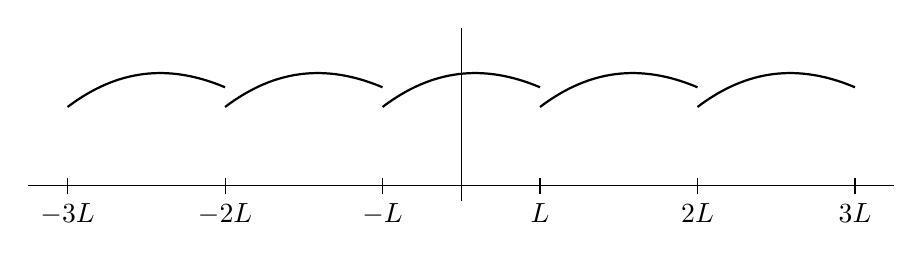
\begin{tikzpicture}
			\draw (0,-0.2) -- (0,2);
			\draw (-5.5,0) -- (5.5,0);
			
			\draw (-5,0.1) -- (-5,-0.1) node[below] {$-3L$};
			\draw[thick] (-5,1) to[bend left] (-3,1.25);
			
			\draw (-3,0.1) -- (-3,-0.1) node[below] {$-2L$};
			\draw[thick] (-3,1) to[bend left] (-1,1.25);
			
			\draw (1,0.1) -- (1,-0.1) node[below] {$L$};
			\draw (-1,0.1) -- (-1,-0.1) node[below] {$-L$};
			\draw[thick] (-1,1) to[bend left] (1,1.25);
			
			\draw (3,0.1) -- (3,-0.1) node[below] {$2L$};
			\draw[thick] (1,1) to[bend left] (3,1.25);
			
			\draw (5,0.1) -- (5,-0.1) node[below] {$3L$};
			\draw[thick] (3,1) to[bend left] (5,1.25);
		\end{tikzpicture}
	\end{center}
	
	\begin{thm}{(Convergence for Fourier Series).}
		If $ f(x) $ is piecewise smooth on $ -L \leq x \leq L $, then the Fourier series of $ f(x) $ converges: 
		\begin{enumerate}[label=\arabic*.)]
			\item To the periodic extension of $ f(x) $, wherever the periodic extension is continuous. 
			\item To the average of the left and right limits, usually 
			\[
				\frac{1}{2} (f(x^-) + f(x^+))
			\]
			where the periodic extension has jump discontinuities.
		\end{enumerate}
	\end{thm}
	
	\subsection{Fourier Sine and Cosine Series}
	
	The Fourier series for an odd function only has sine terms. Thus
	\[
		f(x) \sim \sum\limits_{n=1}^{\infty} B_n \sin\left( \frac{n\pi x}{L} \right)
	\]
	where
	\[
		B_n = \frac{2}{L} \int_0^L f(x) \sin\left( \frac{n\pi x}{L} \right) \, dx
	\]
	Assume now $f(x)$ is given, $0\leq x\leq L$. What does $\sum_{n=1}^{\infty}B_n\sin\left(n\pi x/L \right) $ converge to?

	Define the odd extension of $f$: 
	





\end{document}